% !TEX root = cs224_final_paper.tex

\subsection{Author mixing}\label{subsec:author_mixing}

TODO: Explain the issue with having different authors and put picture here.

\subsection{Notation}

Our corpus $(P,A)$ consists of a set of papers $P=\{p_1, \dots, p_N\}$ and a set of authors $A=\{a_1, \dots, a_K\}$.
Each paper $p_i$ is divided into sentences $s_j^i \in p_i$ that we assume were written by a single author $\mathtt{author_s}(s_j^i)=a_k$.
Alternatively, we could model one author per paragraph or section but it is less clear that such assumptions would hold in practice.
While we assume that a sentence is written by a single author we do not actually observe author labels on sentence level.
We only observe paper level authors and assume that the sentence author is one of the paper authors.
Mathematically, given paper level annotation $\mathtt{author_p}(p_i)=\{a_1, a_7, a_9\}$ we assume 
$$\forall s_j^i\in p_i: \mathtt{author_s}(s_j^i) \in \mathtt{author_p}(p_i)$$

Our goal is to learn to differentiate author styles from the ambiguous ground truth labels $\mathtt{author_p}$ such that we can assign each sentence in a paper to a single author.

We represent this mapping from sentence to author as a matrix $M$ that, for all sentences, contains the single author that is believed to have written that sentence, e.g. $M(s_j^i)=a_k$.
The authors' individual styles are captured through parameters $\theta=(\theta_1, \dots, \theta_K)$ that includes an independent parameter vector for each author $a_k \in A$.

\subsection{Sentence authorship model}
The core of our model describes how likely a given author $a$ is to have generated a given sentence $s$, $p(a|s)$.
We represent a sentence through features $F(s) \in \mathcal{R}^n$ (for more details on our features please refer to section \ref{sec:features}).
We use the following logit model:
\begin{align*}
p(a|s) &=& \operatorname{logit}^{-1}(\langle\theta_a, F(s)\rangle) \\
&=& \frac{1}{1+ \exp({-\langle\theta_a, F(s)\rangle}})
\end{align*}


Note that this model formulation is equivalent to a log-linear model:
$$\log p(\mathtt{author_s}(s)=a | s) = \langle\theta_a, F(s)\rangle - \log Z$$
where $Z$ is a normalizing constant 
$$Z= 1 + \exp(\langle\theta_a, F(s)\rangle).$$

Further note that we have $K$ of these models, one for each author.


\subsection{Learning to differentiate author styles from ambiguous labels}
\label{subsec:fancy_training}

\begin{figure*}[htbp]
\begin{center}
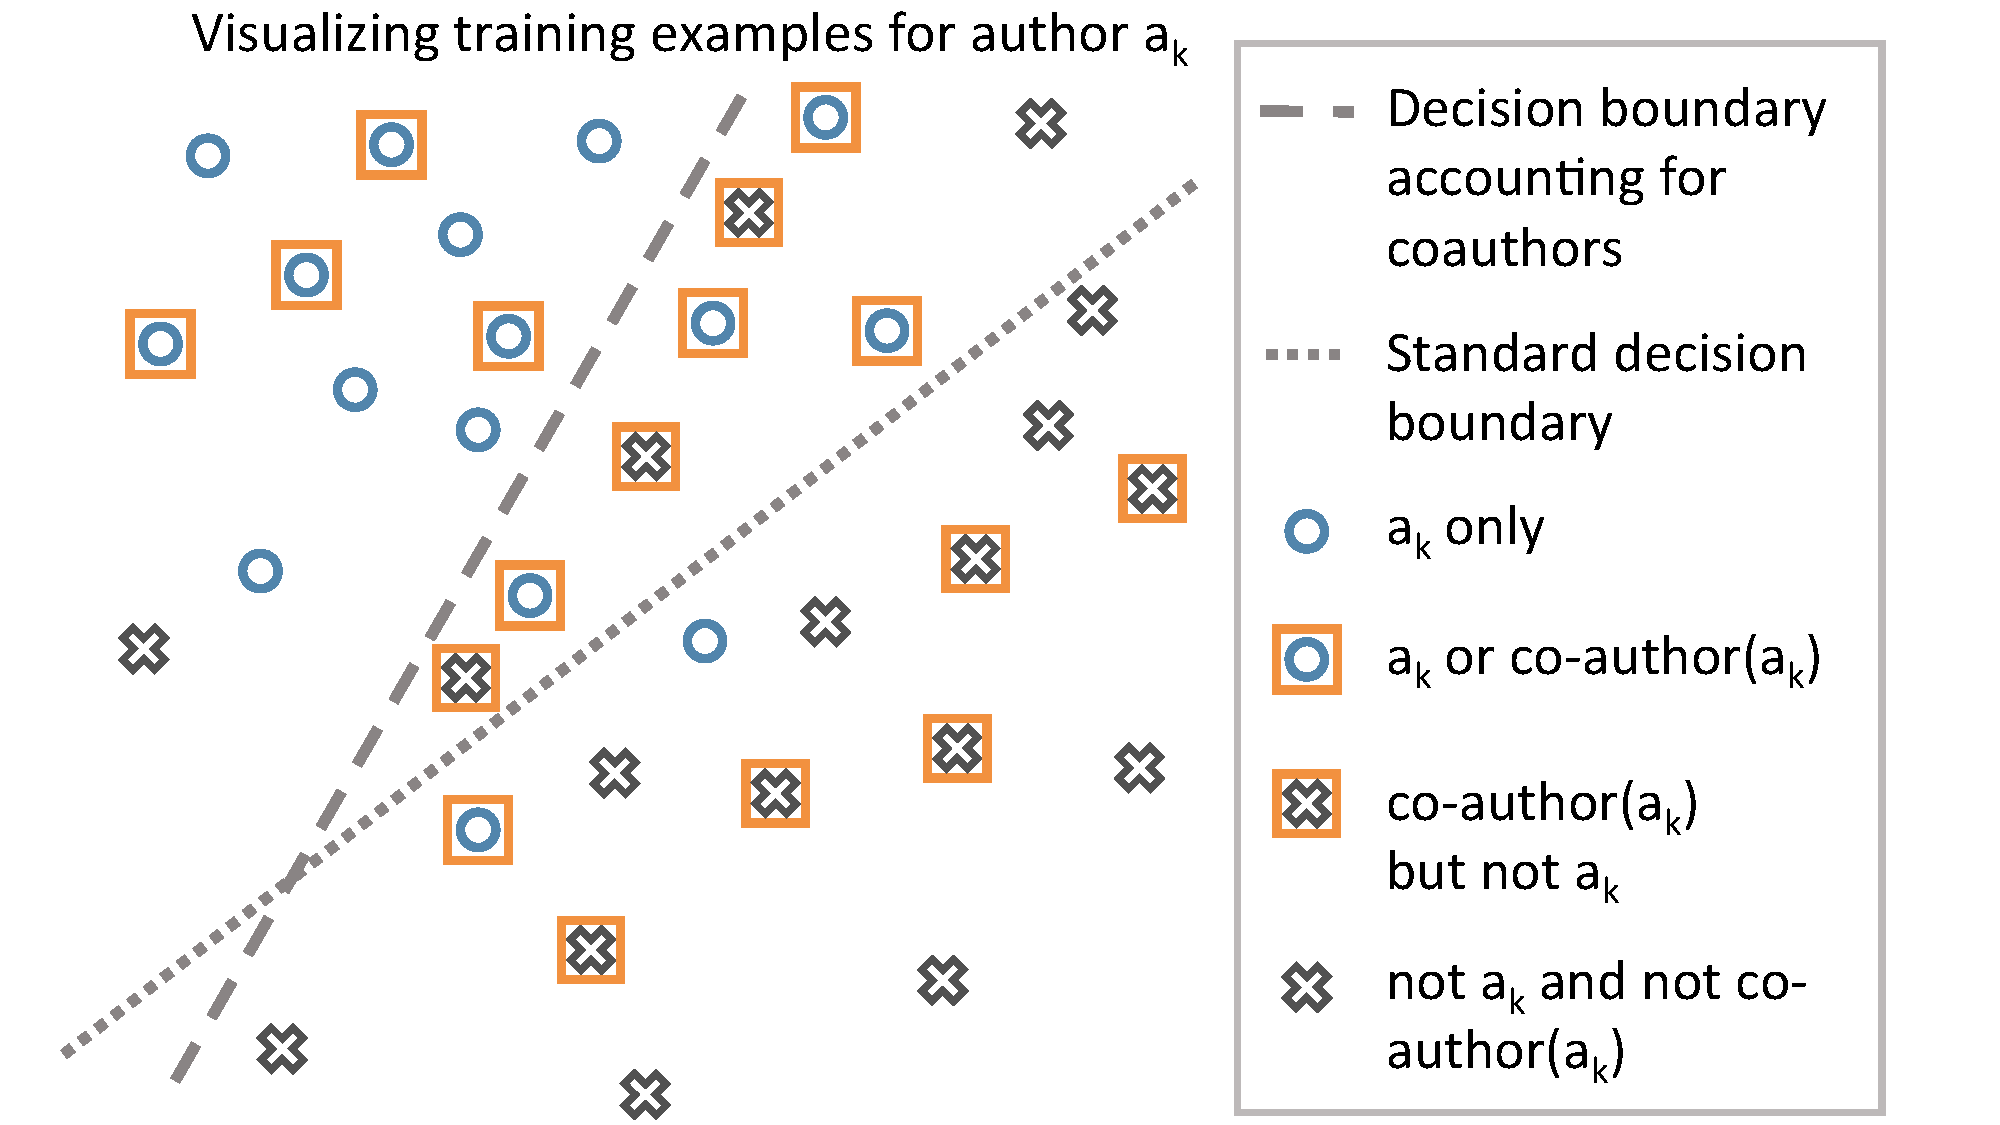
\includegraphics[width=\linewidth]{fancy_training.pdf}
\caption{Training procedure considering co-author negative examples in addition to random negative examples}
\label{fig:fancy_training}
\end{center}
\end{figure*}


A core challenge in learning such logit models is that we lack sentence-level author labels.
As described above, we only observe paper level author labels, i.e. $\mathtt{author_s}(s_j^i) \in \mathtt{author_p}(p_i)$ but we have no basis for assuming any concrete author yet.

Let the authors of a paper $p_i$ be $\mathtt{author_p}(p_i) = \{ a_1, a_2\}$.
To train a model for author $a_1$ we need both positive examples (sentences that $a_1$ did write) and negative example (sentences that $a_1$ did not write). 
For any sentence $s_j^i \in p_i$ we do not know whether it was written by $a_1$ or $a_2$, i.e. we have ambigious sentence labels.
Negative examples are much easier to come by, sentences from any paper that $a_1$ did not co-author would provide true negative examples.

Since we have no basis for assuming, a priori, that sentence $s_j^i$ was definitly written by either $a_1$ or $a_2$ we include all sentences that $a_1$ might have written as positive examples when training an author model for $a_1$. 
Obviously, this will include false positive examples that $a_2$ actually wrote and we need to make sure that we train a model that captures $a_1$'s style and not the combined style of $a_1$ and $a_2$.
To this end, we propose to carefully select negative examples that differentiate $a_1$'s style from the one of $a_2$.
We can achieve this by including positive examples from $a_2$ in as negative examples for $a_1$ (only those sentences that $a_1$ certainly did not write).
In fact, we do not only include but positive examples from all co-authors of $a_1$.
This idea is visualized in Figure \ref{fig:fancy_training}.

In the following, we describe this idea more formally.
We denote the set of all coauthors of a given author $a_k$ by 
\begin{align*}
\mathtt{coauthor}(a_k) =  \{ &a_l \in A \;|\; \forall p\in P: \\
a_l \in \mathtt{author_p}(p) & \Rightarrow a_k \in author_p(p) \}
\end{align*}

Formally, we use the following set of positive examples for $a_k$:
$$ \mathtt{POS}(a_k) = \{ s_j^i \in p_i \;|\; a_k \in \mathtt{author_p}(p_i)\}$$

And the following set of negative examples for $a_k$:
\begin{align*}
\mathtt{NEG}(a_k) = \{ s_j^i \in p_i \;|\; \exists  a_l \in \mathtt{coauthor}(a_k): \\
 a_l \in \mathtt{author_p}(p_i) \wedge a_k \notin \mathtt{author_p}(p_i) \}
\end{align*}

We further add random sentences to $\mathtt{NEG}(a_k)$ since authors have a varying number of co-authors and those with few would end up with very few negative examples otherwise.
%This way of training will be contrasted to just using random negative examples in Section TODO.

\subsection{Refining author models through Expectation Maximization}
Modeling authorship on sentence level gives us the opportunity to further refine our author models (this is not possible on paper level).
The approach described above uses all sentences that could possibly have been written by author $a_k$ as positive examples (recall $\mathtt{POS}(a_k)$).
However, this will include many sentences that were actually written by  one of $a_k$'s coauthors.
Based on our confidence about which sentences were likely written by $a_k$ we can filter the positive examples to yield a cleaner set of positive examples for $a_k$.
We now formalize this intuion.

For the likelihood of the full corpus $(P,A)$ we treat each sentence independently:
$$P(M,\theta | P,A) = \prod_{p_i \in P} \prod_{s_j^i \in p_i} p(M(s_j^i) | s_j^i).$$

The parameter inference problem then becomes
$$\hat{M},\hat{\theta} = \operatorname{argmax}_{M,\theta} P(M,\theta | P,A) - \Omega(M,\theta),$$
where $\Omega(M,\theta)$ is a regularizer on the parameters to avoid overfitting.

Since this optimization depends on both $M$ and $\theta$ we proceed by coordinate ascent on $(M, \theta)$, i.e. by alternately optimizing
$$M^i = \operatorname{argmax}_{M} P(M,\theta^i|A,P)$$
and
$$\theta^{i+1} = \operatorname{argmax}_{\theta} P(M^i,\theta|A,P)$$
until convergence, i.e. until $M^i$ differs from $M^{i-1}$ on less than a prespecified number of sentences (alternatively, one can alternate for a constant number of iterations).

Being a local optimization procedure, coordinate ascent is sensitive to initialization.
Therefore, we initialize the style parameters for each author $\theta^{0}$ by training independent logistic regression models using all sentences an author could have possibly written as positive examples and sentences by his co-authors that he could not have written as well as random other sentences by other authors as negative examples (as formally described in Section \ref{subsec:fancy_training}).

Optimizing for $M$ then is a simple inference step where we dependently assign each sentence to the most likely possible author:
$$M(s_j^i) = \operatorname{argmax}_{a} p(a|s_j^i, \theta)$$

Based on this assignment, optimizing for $\theta$ then becomes estimating $K$ independent logistic regression models for all authors based on the assignment $M$.


\subsection{Predicting paper authors from sentence authors}
Our proposed model gives us predictions on sentence-level $M(s_j^i)$.
While those sentence-level predictions are interesting in its own right (e.g. to estimate contribution of different authors) we ultimately want to predict authors on paper-level.
To this end, we aggregate our sentence-level predictions to paper level predictions by having each sentence $s_j^i$ vote for its most likely author (namely, $M(s_j^i)$).

Compared to this hard voting scheme we also experimented with a soft voting scheme where each author gets a fractional vote depending on their confidence to have written this particular sentence.
However, empirically we found that soft-voting across all sentences of a paper suffers from the same problems that paper-level predictions do \ref{subsec:author_mixing}. 
Hard voting performed better in all test cases.